\section{Introduction}
\label{sec:introduction}

In modern data centers, the efficient utilization of resources is crucial for optimal performance and cost-effectiveness. One of the challenges faced by these systems is the presence of stranded memory, which refers to the allocated but unused memory on remote nodes as seen in Figure \ref{fig:Stranded_memory}, there is over 30\% of the memory is stranded. This stranded memory often coexists with overUtilized CPUs, leading to an imbalance in resource utilization. To address this issue, we propose ImageHarbour, a novel image caching mechanism that aggregates stranded memory from multiple hosts into a single, large memory pool.

\begin{figure}[h]
    \centering
    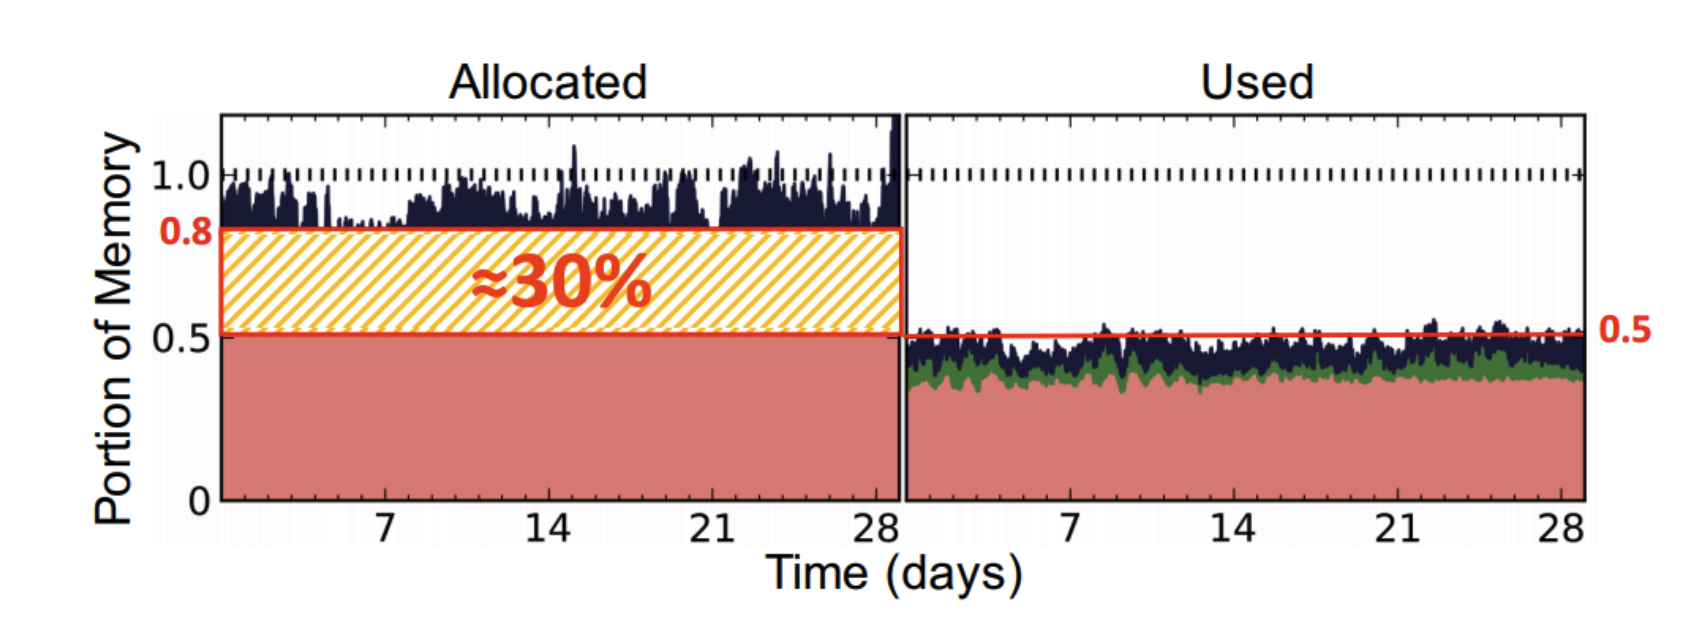
\includegraphics[width=0.4\textwidth]{Stranded_memory.png}
    \caption{stranded memory}
    \label{fig:Stranded_memory}
\end{figure}

ImageHarbour draws inspiration from two key concepts: stranded memory and efficient memory disaggregation. The notion of stranded memory is derived from the study by Reiss et al. \cite{reiss2012heterogeneity}, which highlights the presence of allocated but unused memory in Google's data centers. Their analysis reveals that while some nodes have high CPU utilization, their memory remains underutilized, resulting in stranded memory. On the other hand, the idea of efficient memory disaggregation is borrowed from the work of Gu et al. \cite{gu2017efficient}, which proposes Infiniswap, a remote memory paging system that leverages one-sided Remote Direct Memory Access (RDMA) operations to access memory on remote nodes without interrupting the CPU.

RDMA is a high-performance networking technology that allows direct memory access from the memory of one computer to that of another without involving either computer's operating system \cite{kalia2016design}. This enables low-latency and high-bandwidth communication between nodes in a data center. By exploiting one-sided RDMA operations, ImageHarbour can efficiently access memory on remote nodes with minimal overhead, achieving latencies in the sub-microsecond range. In contrast, traditional disk-based storage systems have latencies around 5-10 milliseconds for a 4KB read operation \cite{yang2014don}, while retrieving Docker images over the internet can take seconds to minutes, depending on the image size and network conditions \cite{harter2016slacker}.

ImageHarbour leverages these concepts to create a distributed image caching system that can significantly improve the performance of image-based workloads in data centers. By pooling together stranded memory from multiple hosts, ImageHarbour creates a large, unified memory pool that can be used to cache frequently accessed Docker images. The system employs a control plane that intelligently manages the cache, deciding which images to bring in, which images to evict, and serving metadata to clients regarding the location of images within the memory pool.

Clients accessing the cached images through ImageHarbour experience significantly reduced latencies compared to traditional image retrieval methods. By serving images directly from memory using one-sided RDMA operations, ImageHarbour can achieve up to 83X lower latency compared to storign the image in the disk and upto 190X lower latency compared to downloading images over the internet.
